% !TEX program = xelatex
\documentclass[11pt,letterpaper]{article}

\usepackage[top=0.8in,bottom=0.85in,left=0.9in,right=0.9in]{geometry}
\usepackage{fontspec}
\usepackage{unicode-math}
\setmainfont{Latin Modern Roman}[Extension=.otf,UprightFont=lmroman10-regular,BoldFont=lmroman10-bold,ItalicFont=lmroman10-italic,BoldItalicFont=lmroman10-bolditalic]
\setsansfont{Latin Modern Sans}[Extension=.otf,UprightFont=lmsans10-regular,BoldFont=lmsans10-bold,ItalicFont=lmsans10-oblique]
\setmonofont{Latin Modern Mono}[Extension=.otf,UprightFont=lmmono10-regular,ItalicFont=lmmono10-italic,Scale=0.85]
\usepackage{xcolor}
\usepackage{titlesec}
\usepackage{enumitem}
\usepackage{fancyhdr}
\usepackage{hyperref}
\usepackage{xurl}
\usepackage{ragged2e}
\usepackage{microtype}
\usepackage{booktabs}
\usepackage{tabularx}
\usepackage{array}
\usepackage{graphicx}
\usepackage{../ac-paper-essay}

\hypersetup{colorlinks=true,linkcolor=acpurple,urlcolor=acpurple,pdfauthor={Jeffrey Alan Scudder and Aesthetic Computer},pdftitle={Pollock-Krasner Application Briefing}}
\pagestyle{fancy}
\fancyhf{}
\renewcommand{\headrulewidth}{0pt}
\fancyhead[L]{\footnotesize\color{acgray} Pollock-Krasner Application Briefing}
\fancyhead[R]{\footnotesize\color{acgray} \thepage}
\setlength{\parindent}{0pt}
\setlength{\parskip}{0.45em}
\linespread{1.08}
\setlist[itemize]{leftmargin=1.3em,itemsep=0.18em,topsep=0.25em}
\newcommand{\status}[1]{\textcolor{acpink}{\textbf{#1}}}
\newcommand{\todo}{\textcolor{acpink}{\fbox{\rule{0pt}{0.55em}\rule{0.55em}{0pt}}}}

\begin{document}
\thispagestyle{empty}
\vspace*{0.35in}
\essaytitle{Pollock-Krasner}
\begin{center}
{\fontsize{18pt}{22pt}\selectfont\color{acdark}Application Briefing}\par
\vspace{0.7em}
{\large\itshape\color{acgray}What is ready, what the record supports, and what must be found}\par
\vspace{1.1em}
{\normalsize Jeffrey Alan Scudder}\par
{\small\color{acgray}Aesthetic Computer papers stack · 20 July 2026}\par
\vspace{1.4em}
{\color{acpink}\rule{0.72\textwidth}{1.2pt}}
\end{center}

\vfill
\begin{quote}
\large
The career is real. The application is started. The unresolved question is narrower: can we document ten qualifying exhibitions and ten recent physical works precisely enough to make a truthful Pollock-Krasner application?
\end{quote}
\vfill
\begin{center}
{\small\color{acgray}Internal working document · not for submission}\par
\end{center}
\clearpage

\section{Executive read}

The Pollock-Krasner Foundation accepts applications year-round from professional visual artists working primarily in painting, sculpture, or works on paper. Awards are unrestricted, up to \$50,000, with most grants around \$35,000. The current working request is \$35,000.

Jeffrey's record supports a serious application: a Fine Art BFA, a Yale MFA, solo and group exhibitions, residencies, teaching, press, institutional presentations, and work held by KADIST and reportedly SMK. His practice has a coherent painter-to-toolmaker arc. Painting came first; software grew from an attempt to make the computer respond with the immediacy of a mark on a surface.

\status{The application is not submission-ready.} The repository does not yet contain a verified inventory of ten eligible physical works. It also does not prove that ten exhibitions in the last decade meet PKF's definition. The public CV describes the 2026 Venice Family Clinic presentation as Jeffrey's first gallery exhibition of physical work in eight years. That gap is an eligibility and competitiveness issue to investigate, not a sentence to write around.

\section{What has been completed}

\begin{itemize}
\item PKF's live guidelines and FAQ were checked against the old Deadlines record.
\item The Deadlines entry was corrected and moved to \textbf{Drafting}.
\item The exact attachment, image, naming, reference, and portal rules were recorded.
\item A working application draft, career audit, exhibition audit, portfolio table, reference table, and output checklist were created.
\item Jeffrey's canonical CV, public biography, papers platter, Jeffrey platter, Whistlegraph platter, prior grant applications, and relevant git history were reviewed.
\item Three independent research passes audited career evidence, application voice, grant precedent, physical-work evidence, and commit provenance.
\item Claims that remain unsupported were deliberately left unresolved rather than filled with plausible language.
\end{itemize}

\section{Application requirements}

\begin{tabularx}{\textwidth}{>{\bfseries}p{0.28\textwidth}X}
\toprule
Item & Current state \\
\midrule
Online application & Not opened; avoid starting the 120-day inactivity clock prematurely \\
Cover letter & Structure drafted; purpose and real figures still needed \\
Artist statement & Painter-centered opening drafted; depends on the ten selected works \\
Résumé / CV & Canonical source exists; needs PKF-specific audit and reconciliation \\
Image list & Template exists; no verified object data entered \\
Ten JPEGs & Not assembled; each must be exactly 2100 px on its longest side \\
Three references & Candidates exist; no final three or confirmed contact details \\
\bottomrule
\end{tabularx}

\clearpage
\section{The strongest truthful spine}

\subsection{Fine-art formation}

Jeffrey earned a BFA in Fine Art from Ringling College of Art and Design in 2011 and an MFA from the Yale School of Art in 2013. Current repo sources describe the Yale concentration as Sculpture; the official credential wording should be confirmed before submission.

\subsection{Pictures crossing screen, paper, and canvas}

Radical Digital Painting began from a painter's standard: the directness of a mark. The practice moved through custom paint programs, performances, and printed pictures. The clearest eligible historical anchor is the 2018 Johannes Vogt Gallery exhibition, documented in the public biography as large-format digital prints on paper.

Whistlegraph continued the drawing thread through scores, sketchbooks, fountain pen, construction paper, manuscripts, and collaborative live performance. Its institutional record includes Rhizome/New Museum and Feral File. These materials may strengthen the story, but each physical object requires sole-versus-collaborative authorship and object metadata before it can enter the portfolio.

The recent return is studio painting on canvas and board, with Turbo Cheap in 2025 and the Venice Family Clinic Art Exhibition in 2026. One repo piece identifies a Jeffrey drawing connected to the VFC auction. Its physical medium and dimensions are not recorded locally.

\subsection{The sentence worth keeping}

\begin{quote}
Painting came first. I trained in fine art at Ringling and in sculpture at Yale, and I never left the standard it set: a mark should feel immediate, physical, and mine.
\end{quote}

That is the right opening because it is plain, personal, and supported by the record. The application should then stay with the visible ten works. Aesthetic Computer belongs in one short paragraph as the long experiment that sharpened Jeffrey's commitment to gesture, authorship, and material response.

\section{Career evidence already in hand}

\begin{itemize}
\item Solo exhibitions recorded at Feral File, Newsstand Project/CAP, left.gallery, Whitcher Projects, Essex Flowers, and SCREEN\_.
\item Group exhibitions recorded at Venice Family Clinic, Turbo Cheap, Internet Archive, 650mAh, Naming Gallery, Johannes Vogt, ZKM, February Gallery, and Neumeister Bar-Am, among others.
\item Residencies recorded at UCLA Social Software, Gazell.io, and Schloss-Post/ZKM; Internet Archive AIR appears in a submitted LACMA CV and should be reconciled into the canonical CV.
\item Teaching at UCLA, Parsons, Southern Oregon University, and Yale workshops.
\item Press and profiles from KADIST, Dirt, Feral File, The Creative Independent, Are.na, Rhizome, Schlosspost, and Artsy.
\item KADIST has a concrete artwork-profile link. The SMK collection claim needs a direct accession or object record.
\end{itemize}

\clearpage
\section{Candidate exhibition audit}

The following list is a research queue, not a claim that the threshold has been met.

\small
\begin{tabularx}{\textwidth}{p{0.08\textwidth}p{0.31\textwidth}X}
\toprule
Year & Exhibition / venue & Missing proof \\
\midrule
2026 & Venice Family Clinic Art Exhibition & Occurrence, checklist, object title, medium, dimensions \\
2025 & Turbo Cheap, Los Angeles & Venue status and exact work shown \\
2019 & Internet Archive AIR Exhibition & Whether eligible physical work was exhibited \\
2018 & \textit{drawings}, 650mAh & Venue status, authorship, media \\
2018 & Naming Gallery, Oakland & Exact work and medium \\
2018 & Johannes Vogt Gallery, New York & Titles, print dimensions, editions \\
2018 & OPEN CODES, ZKM & Exact work and whether PKF counts its medium \\
2018 & RDP: LA, Newsstand Project + CAP & Venue status and objects shown \\
2017 & February Gallery, Austin & Exact work and medium \\
2017 & \textit{New Dawn}, Neumeister Bar-Am & Exact work and medium \\
2017 & \textit{Imaginary Screenshots}, Whitcher Projects & Exact work and medium \\
\bottomrule
\end{tabularx}
\normalsize

Online-only exhibitions, email exhibitions, lectures, and performances should not be counted without written confirmation from PKF. Digital exhibitions may still count toward professional history, but the guidelines do not answer that question clearly enough to assume.

\section{The ten-work inventory}

Every candidate must have all eight fields below before portfolio sequencing begins.

\begin{enumerate}
\item Professional title.
\item Completion year, within the last ten years.
\item Precise eligible medium.
\item Physical dimensions.
\item High-resolution source photograph.
\item Current owner or location.
\item Exhibition history.
\item Sole or collaborative authorship.
\end{enumerate}

At least eight images must show separate works. No more than two may be details, alternate views, or installation views. The ten JPEGs must be exactly 2100 pixels on the longest edge, 72 or 96 DPI, high quality, and named \texttt{Scudder\_Jeffrey\_1.jpg} through \texttt{Scudder\_Jeffrey\_10.jpg}.

\clearpage
\section{Visual research: ten recovered leads}

\begin{center}
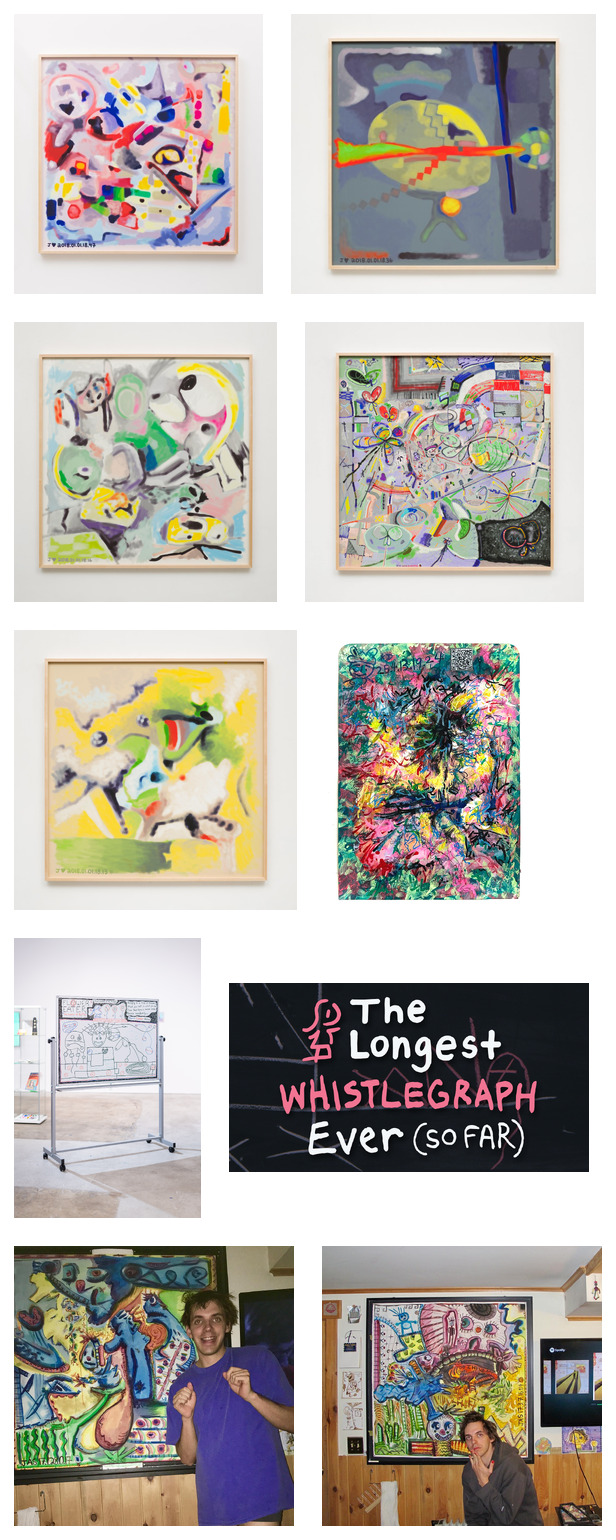
\includegraphics[height=0.72\textheight,keepaspectratio]{../../grants/pollock-krasner-2026/visual-research/contact-sheet.jpg}
\end{center}

This is a discovery sheet, not the recommended final portfolio. The first five images are the documented Johannes Vogt prints; the sixth is the recent Venice Family Clinic work; the seventh is the Internet Archive whiteboard; the eighth is a project cover for \textit{The Longest Whistlegraph Ever (so far)}; and the final two are unidentified physical paintings recovered through Jeffrey's platter.

\clearpage
\section{Artwork-by-artwork assessment}

\small
\begin{tabularx}{\textwidth}{>{\bfseries}p{0.05\textwidth}p{0.30\textwidth}X}
\toprule
No. & Work & Assessment \\
\midrule
1 & \textit{J$\heartsuit$ 2018.01.01.18.47}, 2018. Digital print, 52 $\times$ 52 in. & Strong individual image, title, dimensions, and exhibition record. Confirm that PKF accepts this form of digital painting as work on paper. \\
2 & \textit{J$\heartsuit$ 2018.01.01.18.36}, 2018. Digital print, 52 $\times$ 52 in. & Strong; same eligibility question and same visual series. \\
3 & \textit{J$\heartsuit$ 2018.01.01.18.16}, 2018. Digital print, 52 $\times$ 52 in. & Strong; same eligibility question and same visual series. \\
4 & \textit{J$\heartsuit$ 2018.01.03.19.30}, 2018. Digital print, 52 $\times$ 52 in. & Strong; especially dense bridge between diagram, figure, and painted field. \\
5 & \textit{J$\heartsuit$ 2018.01.01.18.13}, 2018. Digital print, 52 $\times$ 52 in. & Strong; the lightest work in the series and useful for pacing. \\
6 & \textit{25.4.13.19.24}, 2025/2026 exhibition. & Likely the strongest recent work. Recover its exact medium, dimensions, title credit, owner, and a clean high-resolution photograph. \\
7 & \textit{Flower Eater: The Essence of Kid Pix}, whiteboard drawing/diagram, 2019. & Clearly an exhibited physical drawing. Confirm title, marker materials, whiteboard dimensions, ownership, and whether PKF regards it as an autonomous work rather than exhibition interpretation. \\
8 & \textit{The Longest Whistlegraph Ever (so far)}, 2021--2022. & Define the submitted object as the physical full graphic score or a manuscript, not the video/performance. Credit Alex Freundlich, Camille Klein, and Jeffrey Scudder accurately. \\
9 & Platter physical painting lead A; image posted 2017-01-28. & Find the object. The photo suggests a framed physical painting, but title, work date, medium, dimensions, authorship, and location are unknown. \\
10 & Platter physical painting lead B; image posted 2017-03-07. & Find the object. Same unresolved metadata; not yet an application image. \\
\bottomrule
\end{tabularx}
\normalsize

\section{What the images say}

The five Johannes Vogt works form the clearest coherent sequence currently recovered. They share square scale, pale frames, layered marks, diagrammatic figures, soft digital color, and hard-edged strokes. The picture behaves as both field and interface. The gallery's photographs are clean enough for research and supply exact object data, although higher-resolution originals should be recovered for submission.

The Venice Family Clinic work continues that vocabulary while making it materially denser. Its rounded rectangular support, accumulated surface, handwritten date, and embedded QR code distinguish it from the 2018 prints. It is the most convincing bridge back to current studio work.

The Internet Archive photograph is strong because the mobile whiteboard is fully visible as an object. Its black, blue, and red marker drawing is legible and the wheeled support establishes scale. The unresolved question is categorical: drawing, sculpture, diagram, or exhibition interpretation.

The Rhizome archive contains abundant manuscript, blackboard, score, and installation material. The current sheet uses only the microsite cover as a locator. A final portfolio should replace it with one straight, evenly lit photograph of the complete score or manuscript and, only if needed, one installation view. It is a collaborative work and should occupy one work slot.

The final two photographs prove that additional physical paintings exist in Jeffrey's visual history. They are retrieval prompts, not evidence for object data.

\section{Provisional image sequence}

\begin{enumerate}
\item Open with the strongest 2025/2026 physical painting.
\item Add two more recent canvas or board works to establish a sustained return.
\item Use two or three Johannes Vogt prints to establish the earlier visual language.
\item Include the \textit{Meeting Mr. Kid Pix} whiteboard if PKF confirms eligibility.
\item Include the complete \textit{Longest Whistlegraph} score as one collaborative work if eligible.
\item Fill the remaining positions with recent physical works, not project screenshots.
\end{enumerate}

A portfolio weighted toward five digital prints and project documentation could reinforce the concern that Jeffrey's primary practice is digital or performative. The final ten should be weighted toward recent canvas, board, sculpture, and paper objects.

\section{Visual sources}

\begin{itemize}
\item \href{https://johannesvogt.nyc/jeffrey-scudder-and-julia-yerger-radical-digital-paintings/}{Johannes Vogt Gallery}: five Jeffrey works with images, titles, year, and dimensions.
\item \href{https://www.artsy.net/show/johannes-vogt-gallery-radical-digital-painting}{Artsy}: exhibition record identifying pictures printed on paper, videos, drawings, and software.
\item \href{https://www.evergoldprojects.com/exhibition/the-internet-archives-2019-artist-in-residency-exhibition-june-29-august-17/}{Ever Gold Projects}: full Internet Archive AIR installation photography.
\item \href{https://blog.archive.org/2019/06/}{Internet Archive}: exhibition announcement naming \textit{Meeting Mr. Kid Pix} and the whiteboard drawing/diagram.
\item \href{https://sites.rhizome.org/the-longest-whistlegraph-ever-so-far/about/}{Rhizome}: manuscripts, blackboards, score materials, recordings, and project history.
\item \href{https://www.newmuseum.org/exhibition/first-look-the-longest-whistlegraph-ever-so-far/}{New Museum}: institutional record and trio credit.
\item \texttt{papers/jeffrey-platter/} and the public Jeffrey platter: source of the two unidentified painting leads.
\end{itemize}

\section{Where to look next}

\begin{itemize}
\item Studio and phone photographs of the 2025--2026 canvas/board work.
\item Dropbox and old portfolio drives for 2018 Johannes Vogt print files and checklists.
\item iMessage threads around Turbo Cheap and Venice Family Clinic.
\item Whistlegraph manuscript and score archives for solely authored physical drawings.
\item Venue pages, invitations, invoices, checklists, catalogues, and correspondence for the candidate exhibitions.
\item KADIST and SMK object/accession records.
\end{itemize}

\section{Funding story still needed}

PKF does not require a detailed initial budget, and its current FAQ says decisions are based on artistic merit rather than financial need. The cover letter still needs a specific, believable account of what \$35,000 changes over one year.

The useful categories are studio rent and utilities; painting, sculpture, or works-on-paper materials; fabrication; documentation; framing, crating, transport, and exhibition costs; and protected studio time. Actual figures must come from Jeffrey. No hardship, medical need, debt, rent, or income story should be inferred from the repository.

The cover letter should answer three questions in one page:

\begin{enumerate}
\item What physical body of work is being continued now?
\item What does one uninterrupted year make possible?
\item Why is \$35,000 the right amount?
\end{enumerate}

\section{References}

Casey Reas and Julia Yerger are established reference candidates from prior applications. A third reference should ideally be a curator, gallerist, museum professional, or other visual-art peer who can speak directly to the physical work. Contact information and willingness must be confirmed before portal entry.

\clearpage
\section{Full rough application draft}

What follows is the package I would submit if the object records and eligibility questions resolve cleanly. Bracketed passages are the only parts that still require Jeffrey's facts. The prose is intentionally plain and painter-centered.

\subsection{Working request}

\textbf{\$35,000 in unrestricted support for one year.}

This matches PKF's stated typical award. Increase it only if the real one-year studio, living, material, fabrication, documentation, and exhibition costs support a larger request.

\subsection{Cover letter --- rough full draft}

\begin{quote}
\small
Jeffrey Alan Scudder

Dear Pollock-Krasner Foundation Grant Committee,

I am requesting \$35,000 in unrestricted support for one year of sustained work in my Los Angeles studio. The grant would cover [studio rent and utilities], [painting and works-on-paper materials], [framing, fabrication, transport, and documentation], and the protected time required to complete a focused new body of physical pictures.

Painting came first. I trained in fine art at Ringling and in sculpture at Yale, and I never left the standard it set: a mark should feel immediate, physical, and mine. Over the past decade I have carried that question through pictures printed on paper, drawing systems, collaborative graphic scores, and software I built to make the computer respond more like a surface. After years spent developing and performing those instruments, I have returned publicly to canvas and board. The works I am submitting connect that return to the large-format prints I exhibited at Johannes Vogt Gallery in 2018, the \textit{Meeting Mr. Kid Pix} whiteboard shown at Ever Gold Projects in 2019, and the drawing and score practice that became Whistlegraph.

The ten images show [describe the verified recent body and its visible movement in two sentences]. The oldest works establish the visual language: layered fields, diagrams, figures, and marks that behave like instructions. The newest works make that language heavier and more physical. They accumulate color, handwriting, scratches, corrections, and embedded signs until the surface becomes a record of decisions rather than an image of one instant.

The requested support would let me [state the real before-and-after: keep a studio for twelve months; reduce paid work; produce a named number of paintings; frame and transport them; photograph the completed body]. At the end of the grant year I expect to have completed [specific outcome], with the continuity to let the work change slowly instead of being made between other obligations.

Thank you for considering my application.

Sincerely,

Jeffrey Alan Scudder
\end{quote}

\subsection{Artist statement --- rough full draft}

\begin{quote}
\small
Painting came first. I trained in fine art at Ringling and in sculpture at Yale, and I never left the standard it set: a mark should feel immediate, physical, and mine.

The ten works in this application follow pictures as they move among paper, whiteboard, canvas, and score. I build them by accumulation. A soft field receives a hard line; a figure becomes a diagram; handwriting turns into color; a correction stays visible and becomes the next form. The surface records time as a stack of decisions. Even when a work begins on a computer, I am interested in the point where it becomes a physical picture with scale, edge, texture, and a room around it.

The five 2018 prints shown at Johannes Vogt Gallery treat the square as both a painted field and an interface. Their pale grounds hold translucent washes, pixel-like steps, cartoon bodies, directional marks, and dense knots of drawing. The image does not resolve into one scene. It remains a place where incompatible kinds of marks can meet.

The \textit{Meeting Mr. Kid Pix} whiteboard expands that language into an object. Drawn in black, blue, and red marker, it is part diagram, part creature system, and part account of how a child encounters a paint program. Its wheeled support matters: the drawing can turn, move through a room, be erased, or remain.

\textit{The Longest Whistlegraph Ever (so far)} carries drawing into musical notation. Made collaboratively with Alex Freundlich and Camille Klein, its graphic score teaches a performer how to sing every line as it is drawn. [Replace this paragraph with the exact submitted score object's materials, dimensions, and Jeffrey's authorship role.]

The newest physical work, \textit{25.4.13.19.24}, is denser. Its rounded support is covered with green, pink, yellow, blue, black, and white marks that repeatedly build and interrupt one another. Handwritten time and a QR code sit inside the picture rather than outside it. [Add two or three verified recent canvas/board works here and describe what is visibly changing across them.]

Together the works move from printed pictures toward surfaces that carry more touch, more time, and more evidence of revision. The question across them is simple: how much history can one surface hold while every mark remains alive?

Jeffrey Alan Scudder
\end{quote}

\subsection{Provisional ten-image submission}

If submission had to be assembled from what is recovered today, this is the honest rough set. It is not final because Images 9--10 lack object data, Image 8 is represented by a locator rather than the score, and Images 1--5 require a medium-eligibility answer.

\begin{enumerate}
\item \textit{J$\heartsuit$ 2018.01.01.18.47}, 2018, digital print, 52 $\times$ 52 inches.
\item \textit{J$\heartsuit$ 2018.01.01.18.36}, 2018, digital print, 52 $\times$ 52 inches.
\item \textit{J$\heartsuit$ 2018.01.01.18.16}, 2018, digital print, 52 $\times$ 52 inches.
\item \textit{J$\heartsuit$ 2018.01.03.19.30}, 2018, digital print, 52 $\times$ 52 inches.
\item \textit{J$\heartsuit$ 2018.01.01.18.13}, 2018, digital print, 52 $\times$ 52 inches.
\item \textit{25.4.13.19.24}, 2025, [medium], [dimensions].
\item \textit{Flower Eater: The Essence of Kid Pix}, 2019, marker on mobile whiteboard, [dimensions].
\item \textit{The Longest Whistlegraph Ever (so far)}, 2021--2022, [exact score materials and dimensions], with Alex Freundlich and Camille Klein.
\item [Identify platter physical painting A], [year], [medium], [dimensions].
\item [Identify platter physical painting B], [year], [medium], [dimensions].
\end{enumerate}

The preferable final set replaces at least two Johannes Vogt prints and both unidentified paintings with four verified 2025--2026 canvas/board works.

\subsection{Image identification list --- rough draft}

Each final line must follow this exact structure:

\begin{quote}
\texttt{Jeffrey Alan Scudder, Image \#1, 2018, J-heart 2018.01.01.18.47, 52 x 52 inches, digital print}
\end{quote}

Repeat in exact upload order. Final filename: \texttt{ScudderImageList.docx}.

\subsection{Résumé strategy}

Use the canonical CV as source, then make a PKF-specific version that:

\begin{itemize}
\item separates solo and group exhibitions;
\item lists entries newest first;
\item includes dates and locations;
\item does not mix lectures and performances into exhibitions;
\item reconciles the Internet Archive residency;
\item includes KADIST only with its object link and SMK only after verification;
\item keeps software metrics and startup language out of the foreground.
\end{itemize}

Final filename: \texttt{ScudderResume.docx}.

\subsection{References --- rough slate}

\begin{enumerate}
\item Casey Reas --- artist and UCLA Design Media Arts professor; current residency host and peer. [Confirm email and phone.]
\item Julia Yerger --- artist and Radical Digital Painting collaborator; can address the Johannes Vogt exhibition and Jeffrey's picture-making practice. [Confirm email and phone.]
\item [Visual-art curator, gallerist, museum professional, or collector who knows the recent physical work.] [Confirm role, institution, email, and phone.]
\end{enumerate}

\subsection{Required submission files}

\begin{itemize}
\item \texttt{ScudderCoverLetter.docx}
\item \texttt{ScudderResume.docx}
\item \texttt{ScudderArtistStatement.docx}
\item \texttt{ScudderImageList.docx}
\item \texttt{Scudder\_Jeffrey\_1.jpg} through \texttt{Scudder\_Jeffrey\_10.jpg}
\end{itemize}

\section{Decision gate}

\begin{tabularx}{\textwidth}{>{\bfseries}p{0.32\textwidth}X}
\toprule
Proceed when & Hold when \\
\midrule
Ten eligible objects are documented & The portfolio depends mainly on software screenshots or digital originals \\
Ten exhibitions can be defended & The count requires lectures, performances, or online-only events PKF will not accept \\
The recent body is coherent & The ten images are a retrospective sampler without a visual argument \\
Real use-of-funds figures exist & The request remains a generic \$35,000 placeholder \\
Three references are confirmed & References cannot speak to the submitted physical practice \\
\bottomrule
\end{tabularx}

\section{Immediate checklist}

\begin{itemize}
\item[\todo] Ask PKF the exhibition-threshold question in writing.
\item[\todo] Retrieve and photograph ten candidate physical works.
\item[\todo] Verify VFC and Turbo Cheap object details.
\item[\todo] Recover the Johannes Vogt checklist and print specifications.
\item[\todo] Verify the SMK collection record.
\item[\todo] Confirm three references.
\item[\todo] Supply real one-year costs and choose the final request amount.
\item[\todo] Only then create the online application and start its 120-day inactivity clock.
\end{itemize}

\section{Working files}

\begin{itemize}
\item \texttt{grants/pollock-krasner-2026/DRAFT.md}
\item \texttt{grants/pollock-krasner-2026/RESEARCH.md}
\item \texttt{grants/pollock-krasner-2026/CAREER-AUDIT.md}
\item \texttt{papers/cv/cv.tex}
\item \texttt{papers/jeffrey-platter/README.md}
\item \texttt{papers/whistlegraph-platter/README.md}
\end{itemize}

\colophon{Prepared from the Aesthetic Computer monorepo, the papers and platter stacks, prior submitted applications, and git history. This briefing distinguishes repository evidence from claims that still need external documentation.}

\end{document}
